\documentclass[11pt,a4paper]{article}
\usepackage[T1]{fontenc}
\usepackage[utf8]{inputenc}
\usepackage{lmodern}
\usepackage[margin=2.5cm]{geometry}
\usepackage{amsmath,amssymb}
\usepackage{booktabs}
\usepackage{graphicx}
\usepackage[hidelinks]{hyperref}
\hypersetup{pdfauthor={Gianni Pilotti},pdftitle={Markowitz, Black-Litterman and Risk Parity on Ten US Stocks},pdfcreator={},pdfproducer={}}
\setlength{\parindent}{0pt}
\setlength{\parskip}{6pt}

\title{Markowitz, Black-Litterman and Risk Parity on Ten US Stocks}
\author{Gianni Pilotti}
\date{}

\begin{document}
\maketitle

\section{The Core Idea}
The repository builds three long-only portfolios from the same ten US stocks and compares them. The first is a Markowitz mean-variance portfolio, shown at maximum Sharpe ratio and at minimum variance. The second is a Black-Litterman portfolio that combines market equilibrium returns with two investor views. The third is a risk parity portfolio in which every stock contributes the same share of total risk. All three use daily prices from 2019 to 2026 and a risk-free rate of 3\%.

\begin{itemize}
\item \textbf{Same data, different weights:} the maximum Sharpe portfolio puts 70\% in two stocks (NVDA and JNJ), while risk parity keeps every stock between 6.1\% and 14.7\%.
\item \textbf{Returns drive the answer:} the expected returns are historical averages, so the Sharpe ratios are in-sample and optimistic.
\end{itemize}

\section{Method}
\subsection{Data}
Daily adjusted closes come from Yahoo Finance through yfinance, for AAPL, MSFT, JPM, XOM, JNJ, PG, V, NVDA, KO and UNH. The request runs from 1 January 2019 to 1 August 2026, an end date that yfinance treats as exclusive. Rows with any missing close are dropped. This leaves 1,905 prices and 1,904 daily simple returns, from 2 January 2019 to 31 July 2026. Columns are put in the ticker order straight after the download, so weights, covariance matrix and Black-Litterman views refer to the same asset order. With $r$ the vector of daily simple returns, the annualized inputs use 252 trading days:
\[
\mu = 252\,\mathbb{E}[r], \qquad \Sigma = 252\,\mathrm{Cov}(r).
\]

\subsection{Markowitz}
For weights $w$, the expected return is $w^\top\mu$, the volatility is $\sqrt{w^\top\Sigma w}$ and the Sharpe ratio is $(w^\top\mu-r_f)/\sqrt{w^\top\Sigma w}$, with $r_f=3\%$. The maximum Sharpe portfolio solves
\[
\max_w \frac{w^\top\mu-r_f}{\sqrt{w^\top\Sigma w}}
\quad\text{subject to}\quad \sum_i w_i=1,\quad 0\le w_i\le 1,
\]
and the minimum variance portfolio minimizes $w^\top\Sigma w$ under the same constraints. Both use SLSQP from equal weights. The efficient frontier is traced by minimizing variance for 40 target returns spaced evenly between the lowest and highest stock mean.

\subsection{Black-Litterman}
The equilibrium excess return is $\Pi=\lambda\,\Sigma w_m$, with risk aversion $\lambda=2.5$. The market weights $w_m$ are equal, 10\% per stock, as a stand-in for market capitalization. The views sit in a $2\times 10$ matrix $P$ and a vector $Q$. The first view puts $+1$ on NVDA and $-0.5$ on each of AAPL and MSFT, with $Q_1=5\%$. The second puts $+1$ on JPM, with $Q_2=8\%$. The view uncertainty is $\Omega=\mathrm{diag}(P\,\tau\Sigma\,P^\top)$ with $\tau=0.05$, and the posterior mean is
\[
\mu_{BL}=\left[(\tau\Sigma)^{-1}+P^\top\Omega^{-1}P\right]^{-1}\left[(\tau\Sigma)^{-1}\Pi+P^\top\Omega^{-1}Q\right].
\]
The maximum Sharpe portfolio is then solved with $\mu_{BL}$ and the same $\Sigma$.

\subsection{Risk parity}
Stock $i$ contributes $RC_i = w_i(\Sigma w)_i / (w^\top\Sigma w)$ to portfolio variance, and the contributions sum to one. The weights minimize $\sum_i (RC_i-1/10)^2$ subject to the budget constraint $\sum_i w_i=1$ and bounds $0.001\le w_i\le 1$, again with SLSQP.

\section{Results}
\begin{center}
\begin{tabular}{@{}lccc@{}}
\toprule
Portfolio & Expected return & Volatility & Sharpe \\
\midrule
Max Sharpe (Markowitz) & 37.4\% & 25.1\% & 1.37 \\
Min variance (Markowitz) & 15.6\% & 15.8\% & 0.79 \\
Black-Litterman & 30.6\% & 23.8\% & 1.16 \\
Risk parity & 20.9\% & 17.5\% & 1.02 \\
\bottomrule
\end{tabular}
\end{center}

\begin{center}
\begin{tabular}{@{}lcccc@{}}
\toprule
Stock & Max Sharpe & Min variance & Black-Litterman & Risk parity \\
\midrule
AAPL & 10.4 & 0.0 & 19.6 & 8.0 \\
MSFT & 0.0 & 10.3 & 9.3 & 8.6 \\
JPM & 2.5 & 0.3 & 9.8 & 8.5 \\
XOM & 10.3 & 9.7 & 9.6 & 10.0 \\
JNJ & 31.2 & 33.8 & 0.0 & 14.7 \\
PG & 0.0 & 21.9 & 0.0 & 13.4 \\
V & 0.0 & 0.0 & 18.0 & 8.7 \\
NVDA & 39.2 & 1.3 & 18.2 & 6.1 \\
KO & 6.4 & 20.5 & 0.0 & 12.9 \\
UNH & 0.0 & 2.2 & 15.6 & 9.1 \\
\bottomrule
\end{tabular}
\end{center}
Weights in percent, rounded to one decimal from the unrounded solver output.

The maximum Sharpe portfolio holds six stocks, so its weights are sensitive to the estimated means. Black-Litterman gives NVDA 18.2\%, against the 10\% equal prior, and gives no weight to JNJ, PG or KO. Risk parity is the most spread out. Recomputed from the saved weights, its ten risk contributions lie between 9.97\% and 10.03\%, so the solver meets its target.

\begin{figure}[h]
\centering
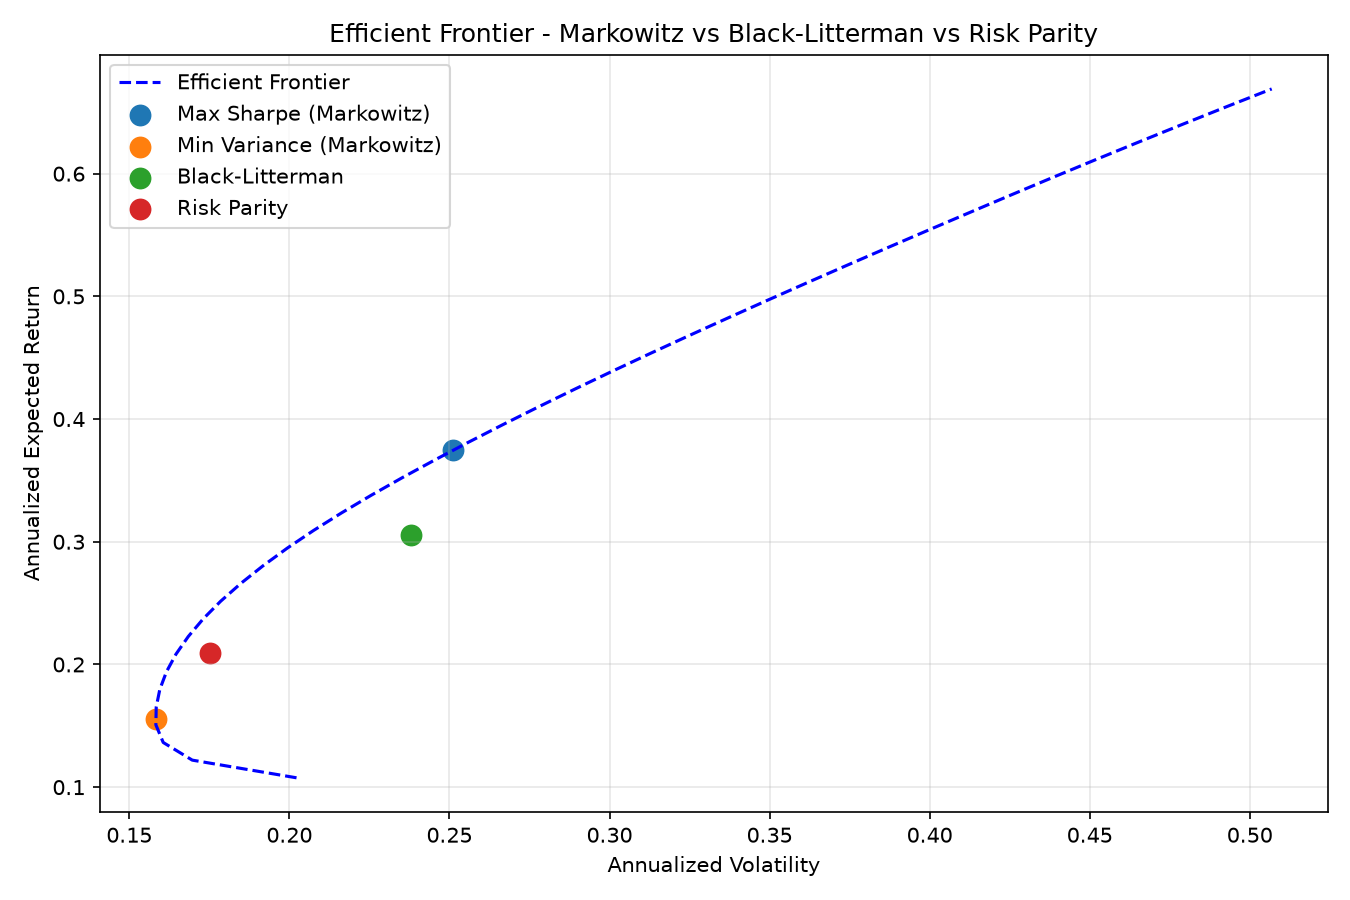
\includegraphics[width=0.85\textwidth]{../output/efficient_frontier.png}
\caption{Efficient frontier (dashed) and the four portfolios, from the repository output.}
\end{figure}

\section{Worked Example}
The maximum Sharpe weights are the four-decimal values in the repository output. The annual means come from the same price download. Each stock adds $w_i\mu_i$ to the expected return, and only six weights are nonzero:
\begin{align*}
\mu_p &= 0.3922\times 0.6691 + 0.3123\times 0.1384 + 0.1035\times 0.3269
 + 0.1029\times 0.1991 \\
&\quad + 0.0644\times 0.1328 + 0.0247\times 0.2387 \\
&= 0.2624 + 0.0432 + 0.0338 + 0.0205 + 0.0086 + 0.0059 = 0.3744.
\end{align*}
NVDA alone adds 0.2624, which is 26.2 points of the 37.4\% expected return. With the stored volatility of 25.1\%, the Sharpe ratio is
\[
\frac{0.3744-0.03}{0.2510} = 1.372 \approx 1.37.
\]
Both figures match \texttt{portfolio\_stats.csv}.

\section{Limits}
\begin{itemize}
\item \textbf{In-sample means:} the expected returns and the risk come from the same history. NVDA's mean of 66.9\% a year supplies most of the maximum Sharpe return, so the result depends on one stock's past.
\item \textbf{Illustrative views:} the two Black-Litterman views are chosen for the example, not forecasts. The posterior weights follow them directly.
\item \textbf{Market weights:} equal weights replace market capitalization in the equilibrium return.
\item \textbf{Mixed return basis:} the equilibrium return is an excess return, while the historical means are total returns. The Sharpe formula subtracts 3\% from both, so the two bases are not reconciled.
\item \textbf{Covariance and solver:} Black-Litterman changes only the mean vector, and risk always uses the historical covariance. SLSQP is a local solver with one starting point, and the code does not check the solver's success flag.
\item \textbf{Scope:} the portfolios are long-only, with no transaction costs and no rebalancing. These are model outputs, not recommendations.
\end{itemize}

\end{document}
